\section{Problema 1.3}

\begin{tcolorbox}
\begin{problema}
	Considere dos fermiones idénticos (ningún nivel de energía puede tener más de una partícula) en un sistema de $2$ niveles de energía, donde las energías son $0$ y $\epsilon$. En términos de $\epsilon$ y $T$ calcular
	\begin{enumerate}
		\item La función partición del ensamble canónico $\zc$
		\item La energía promedio $\ev{E}$. Además ver que sucede con $\ev{E}$ en los límites cuando $T\to 0$ y $T\to\infty$.
		\item La entropía $S$. Analizar los mismo límites para $T$.
		\item Ahora, el sistema es conectado a un baño de partículas con potencial químico $\m$. Calcule $\zgc(\m,T)$. Encuentre el número  de partículas, $\ev{N}$ como función de $\m$ y $T$. Además, calcules los mismo límites anteriores en $T$.
	\end{enumerate}
\end{problema}
\end{tcolorbox}

\begin{sol}
\
\begin{enumerate}
\begin{figure}[h!]
	\centering
	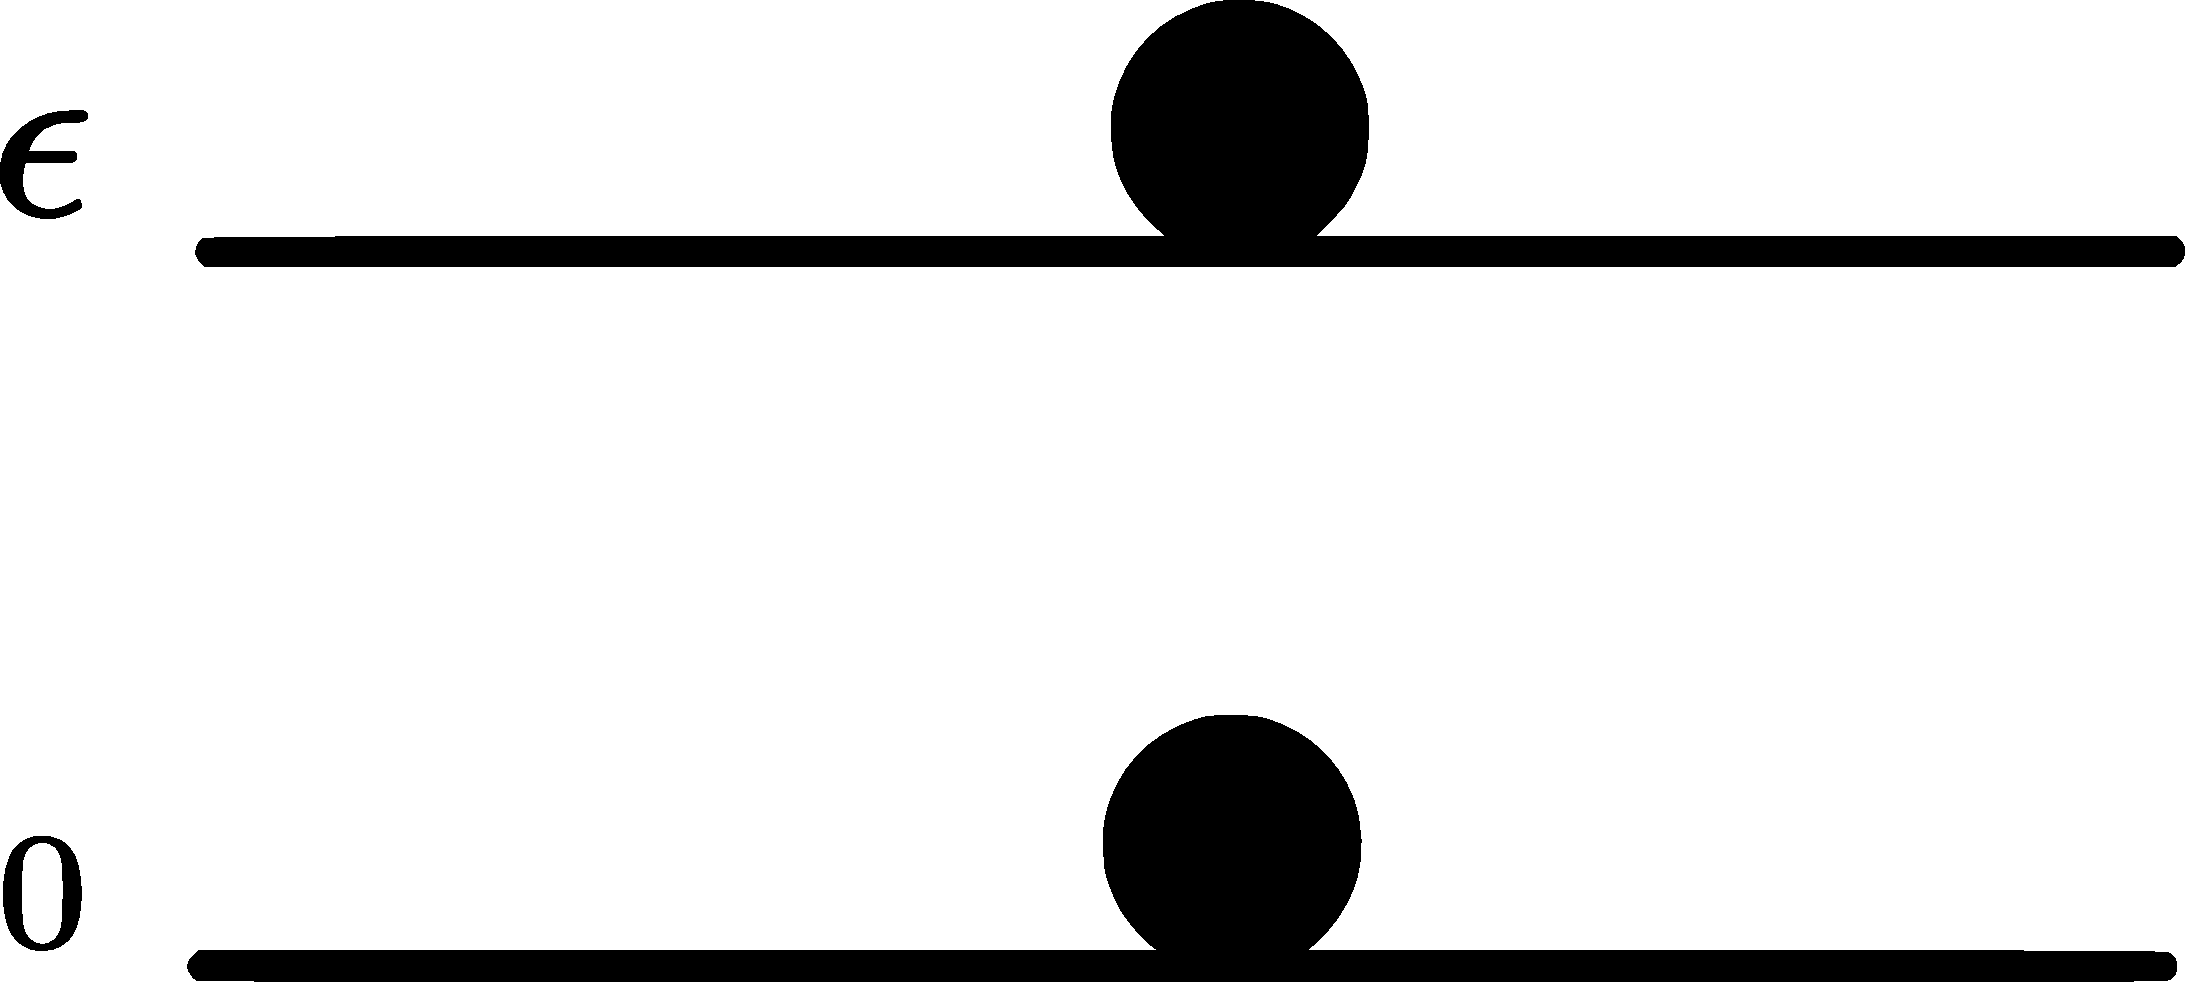
\includegraphics[scale=0.13]{energy-levels.pdf}
	\caption{Única configuración posible para el problema dado.}
	\label{fig:1.3}
\end{figure}	
\item 
Notemos que debido al hecho de que estamos considerando $2$ fermiones idénticos en un sistema de $2$ niveles de energía, existe sólo una configuración posible para el sistema, de manera tal que ningún nivel de energía tengas más de una partícula, representada en la Figura \ref{fig:1.3}.

Sabemos que la función de partición del ensamble canónico viene dada por
\begin{equation}
  \zc=\sumi e^{-\b \epsilon_i},\qquad \b=\frac{1}{\k T}
\end{equation}
Para este caso, tenemos
\begin{align}
  \zc&=e^{-\b \epsilon}\\
 \Aboxed{ \zc&=e^{-\epsilon/\k T}\label{1-Zc}}
\end{align}

\item 
La energía promedio se obtiene como
\begin{align}\label{13-evE}
  \ev{E}=\sumi \epsilon_iP_i
\end{align}
donde
\begin{equation}
	P_i=\frac{e^{-\b \epsilon_i}}{\zc }
\end{equation}
Usando \eqref{1-Zc}, se tiene
\begin{equation}
  P_i=\frac{e^{-\b \epsilon}}{e^{-\b \epsilon}}=1
\end{equation}
así de \eqref{13-evE} , la energía promedio es
\begin{equation}\label{E}
\boxed{  \ev{E}=\epsilon}
\end{equation}
Notemos que esta igual puede ser calculada usando
\begin{align}
  \ev{E}&=-\pdv{\b}\ln (\zc)\\
  &=-\pdv{\b}\ln(e^{-\b \epsilon})\\
  &=-\pdv{\b}(-\b \epsilon)\\
  &=\epsilon
\end{align}
lo cual es consistente con \eqref{E}. Notemos que este valor no depende de $T$, luego
\begin{equation}
  \boxed{\lim_{T\to 0}\ev{E}= \lim_{T\to\infty}\ev{E}=\epsilon}
\end{equation}
Es decir, para cualquier $T$, el valor de expectación de la energía será el mismo. Pero esto es consistente ya que el sistema siempre estará en la única configuración en la cual puede estar, con energía total $\epsilon$.
% todas las configuraciones tienen la misma probabilidad, pero sólo existe una única configuración posible. Luego, el resultado es consistente.

\item 
Para calcular la entropía $S$, notemos que de la energía libre de Hemholtz,
\begin{equation}
  F=\ev{E}-TS=-\k T\ln (\zc)
\end{equation}
podemos despejar $S$,
\begin{equation}
  S=\frac{\ev{E}}{T}+\k \ln(\zc )
\end{equation}
Usando lo encontrado anteriormente, tenemos
\begin{align}
  S&=\frac{\epsilon}{T}+\k (-\b \epsilon)\\
  &=\frac{\epsilon}{T}-\frac{\kappa}{\k T}\epsilon\\
  &=\frac{\epsilon}{T}-\frac{\epsilon}{T}\\
  \implies \Aboxed{S&=0}
\end{align}
Al igual que antes este valor no depende de $T$, luego
\begin{equation}
  \boxed{\lim_{T\to 0}S= \lim_{T\to\infty}S=0}
\end{equation}
Este resultado igual es consistente con lo esperado, ya que al existir sólo un único microestado comptible con  el sistema, $S\sim \ln (1)=0$, independientmenete del valor de $T$.
 %--------0--------
 \item
Debido a que ahora estamos permitiendo que el número de partículas fluctúe, debemos calcular la función partición del ensamble gran canónico $\zgc$ de manera similar al ejercicio realizado en clases para el caso de los bosones. Por definición, $\zgc$ viene dada por
\begin{equation}\label{1.zgc}
  \zgc=\sum_le^{-\b (E_l-\m N_l)}
\end{equation}
donde $l$ es la configuración total del sistema, $E_l$ es la energía total del sistema y $N_l$ corresponde al número de partículas total del sistema. Sea $i$ el número de partículas en el nivel $1$ con energía $0$ y sea $j$ el número de partículas en el nivel $2$ con energía $\epsilon$. Así, se tiene
\begin{align}
  E_l&=0\cdot i+\epsilon\cdot j=\epsilon j\\
  N_l&=i+j
\end{align}
Notar que en este caso, debido a que estamos considerando fermiones, el número de partículas que puede haber en un nivel de energía puede ser únicamente $0$ ó $1$. Luego, \eqref{1.zgc} queda
\begin{align}
  \zgc &=\sum_{i,j}e^{-\b(\epsilon j-\m i-\m j)}\\
  &=\sum_{i=0}^1e^{\b \m i}\sum_{j=0}^1e^{-\b (\epsilon-\m )j}\\
  &=\left(1+e^{\b \m }\right)\left(1+e^{-\b(\epsilon-\m )}\right)\label{1.zgc-exp}
\end{align}
\begin{equation}
	\implies\boxed{ \zgc=\left(1+e^{\m/\k T }\right)\left(1+e^{-(\epsilon-\m )/\k T}\right)}
\end{equation}

Para calcular el número de partículas, usamos
\begin{equation}\label{1.N}
  \ev{N}=-\pdv{\a}\ln(\zgc)=\pdv{(\b\m )}\ln(\zgc)
\end{equation}
De \eqref{1.zgc-exp} se tiene
\begin{align}
  \ln(\zgc)&=\ln \left[\left(1+e^{\b \m }\right)\left(1+e^{-\b(\epsilon-\m )}\right)\right]\\
  &=\ln\left(1+e^{\b \m }\right)+ \ln \left(1+e^{-\b(\epsilon-\m )}\right)
\end{align}
De \eqref{1.N}
\begin{align}
  \ev{N}&=\pdv{(\b\m )}\ln(\zgc)\\
  &=\pdv{(\b \m)  }\left[\ln\left(1+e^{\b \m }\right)+ \ln \left(1+e^{-\b(\epsilon-\m )}\right)\right]\\
  &=\frac{e^{\b\m }}{1+e^{\b \m }}+\frac{e^{-\b (\epsilon-\m )}}{1+e^{-\b(\epsilon-\m )}}
\end{align}
\begin{equation}
	\implies 	\boxed{\ev{N}=\frac{e^{\m/\k T }}{1+e^{ \m/\k T }}+\frac{e^{-(\epsilon-\m )/\k T}}{1+e^{-(\epsilon-\m )/\k T}}}
\end{equation}

Para calcular los límites notemos que para $T\to 0$ habrá una indeterminación tipo $\infty	/\infty$, luego, usamos L'Hopital,
\begin{align}
  \lim_{T\to 0 }\ev{N}&=\lim_{T\to 0}\left\{\frac{e^{\m/\k T }}{1+e^{ \m/\k T }}+\frac{e^{-(\epsilon-\m )/\k T}}{1+e^{-(\epsilon-\m )/\k T}}\right\}\\
  &=\lim_{T\to 0}\left\{\frac{-\dfrac{\m }{\k T^2}e^{\m/\k T}}{-\dfrac{\m }{\k T^2}e^{\m/\k T}}+\frac{\dfrac{k}{T^2}(\epsilon-\m )e^{-(\epsilon-\m )/\k T}}{\dfrac{k}{T^2}(\epsilon-\m )e^{-(\epsilon-\m )/\k T}}\right\}\\
  &=\lim_{T\to 0}\{1+1\}\\
  &=\lim_{T\to 0}\left\{2\right\}\\
  &=2
\end{align}

Por otro lado,
\begin{align}
  \lim_{T\to \infty }\ev{N}&=\lim_{T\to\infty }\left\{\frac{e^{\m/\k T }}{1+e^{ \m/\k T }}+\frac{e^{-(\epsilon-\m )/\k T}}{1+e^{-(\epsilon-\m )/\k T}}\right\}\\
  &=\frac{1}{1+1}+\frac{1}{1+1}\\
  &=\frac{1}{2}+\frac{1}{2}\\
  &=1
\end{align}
\end{enumerate}
%TODO interpretación

















\end{sol}
